\chapter{\psitomotitle: Platform for Seismic Imaging (Deterministic)}
\label{chapter:psi_d}

\section{Overview} \label{PSI_D:Overview}
The Platform for Seismic Imaging (\psitomotitle{}) is a Julia package for performing forward and deterministic inverse modelling of seismic datasets. Another stochastic inversion methodology is under development and planned for a future release (see Del Piccolo et al., 2023). The primary motivation for its development was to facilitate the conversion of mantle geodynamic models into realistic seismic velocity models that may in turn be compared to imaging results from real arrays. This allows one to better understand how geodynamic features may be represented in seismic images and to identify potential artefacts--particularly those arising from neglecting anisotropy \citep[e.g.][]{bezada2016g3, vanderbeek2021, vanderbeek2023}. To this end, synthetic seismic datasets can be generated directly from elastic models produced via \viztomotitle{} (Chapter \ref{chapter:viztomo}) and subsequently inverted for both isotropic and/or anisotropic parameters. Note that only \viztomotitle{} models in spherical coordinates are supported at this time.

At present, \psitomotitle{} can predict P and S travel-times, splitting intensity, and shear wave splitting parameters in a ray-theoretical framework. Forward calculations are supported for models parameterized by (1) isotropic body wave velocities, (2) Thomsen parameters describing hexagonally anisotropic media, and (3) the full 21-component elastic tensor. Travel-time and splitting intensity datasets can be inverted for both isotropic and hexagonally anisotropic 3D models with arbitrary symmetry axis orientations. The inversion is performed using an iterative Gauss-Newton approach to solve for the model perturbations that minimize the sum of the squared data residuals in addition to constraints on the model norm and Laplacian. For a complete description of the methodology see \cite{vanderbeek2021} and \cite{vanderbeek2023}.


\section{Installation} \label{PSI_D:Installation}
\psitomotitle{}, may be installed from Julia's package manager,

\texttt{julia> using Pkg} \\
\texttt{julia> Pkg.add(url="https://github.com/bvanderbeek/PSI\_D.git")}

\textbf{Attention non-Windows users!} For travel-time and ray path calculations, \psitomotitle{} uses the \textbf{TauP Toolkit} [Crotwell et al., 1999]. For the Julia wrapper to this Java program to function properly, the environment variable \texttt{JULIA\_COPY\_STACKS = yes} must be defined. This may be done within the shell configuration file or in Julia prior to loading the \psitomotitle{} package,

\texttt{julia> ENV["JULIA\_COPY\_STACKS"] = "yes"}

\textbf{Attention Mac users!} To avoid Java related segmentation faults, Julia must be started with the flag \texttt{---handle-signals=no}. Note that this may cause multithreading in Julia to crash.

A pure Julia implementation of the travel-time calculations and ray tracing is planned for a future release to avoid these Java-related inconveniences.

\section{Forward Modelling} \label{PSI_D:Forward Modelling}

All the parameters required to make predictions are defined in a TOML file (see \path{https://toml.io/en/}). An example parameter file is located in: \path{examples/SinkingSlab/psi_input/psi_parameters_synthetic.toml}. The TOML table headings and variables are detailed below (\ref{forward_parameters}).

Once the parameter file is defined, predictions can be made by calling the forward problem function with the parameter file as input, e.g.,

\texttt{julia> psi\_forward("psi\_input/psi\_parameters\_synthetic.toml")}

Upon completion of the forward calculation, the predictions will be written to \texttt{csv}-formatted files in the output directory specified in the parameter file. A separate file is generated for each observation and phase (i.e., P or S) pair. The structure of these files is detailed below. A copy of the parameter file used to call \texttt{psi\_forward} will also be saved.

\subsection{Parameter file variables for forward modelling} \label{forward_parameters}
1. \texttt{[Output]}
\begin{itemize}
\item \texttt{output\_directory}: Path (String) to the directory where results are written.
\item \texttt{tf\_time\_stamp}: Flag (Boolean) that when \texttt{true} will write results to a time-stamped folder (\texttt{yymmdd\_hhmmss}) in \texttt{output\_directory}. This is for convenience if one does not want to define unique names for every run.
\end{itemize}
At least one of the following observations types should be defined,

2.1. \texttt{[Observations.TravelTime.CompressionalWave]}
\begin{itemize}
\item \texttt{filename}: Path (String) to file containing P-wave travel-time data. Data should be written to a \texttt{csv}-formatted file with the following columns, travel-time (s), error (s), dominant waveform period (s; this will be used in the future for finite-frequency kernels), IASPEI recognized phase name, source ID (Integer), receiver ID (String), Channel (String; not currently used for any calculations but for reference).
\end{itemize}
2.2. \texttt{[Observations.TravelTime.ShearWave]}
\begin{itemize}
\item \texttt{filename}: Defined as above. However, for anisotropic forward calculations an additional 8$^{\text{th}}$ column containing the polarization azimuth measured counter-clockwise positive from the Q-channel (in ray-aligned QTL-coordinates) should be defined. If not present, shear waves are assumed to be radially polarized.
\end{itemize}
2.3. \texttt{[Observations.SplittingIntensity.ShearWave]}
\begin{itemize}
\item \texttt{filename}: Defined as above for S-wave travel-times (replacing the travel-time and error columns with the splitting intensity values).
\end{itemize}
2.4. \texttt{[Observations.SplittingParameters.ShearWave]}
\begin{itemize}
\item \texttt{filename}: Defined similar to the S-wave travel-time file. However, the first two columns contain the split time (s) and fast-azimuth (radians), respectively. The 3$^{\text{rd}}$ and 4$^{\text{th}}$ columns contain the errors in the split time and fast-azimuth.
\end{itemize}

3.1 \texttt{[Model]}
\begin{itemize}
\item \texttt{parameterisation}: The type of parameterization (String) used to define the velocity model. Options are \texttt{"IsotropicVelocity"},\\ \texttt{"HexagonalVectoralVelocity"} for hexagonal anisotropic models with arbitrary symmetry axis orientations, or \texttt{"ElasticVoigt"} when models are defined using the 21-component elastic tensor.
\item \texttt{theModel}: Path (String) to the \texttt{csv}-file containing model data. At present, models must be defined on a regular grid in spherical coordinates. Each model file must contain 3 header lines,\\
Header 1: Earth radius (km), longitude of model origin (i.e. center; decimal degrees), latitude of model origin (i.e. center; decimal degrees), rotation of model from north (radians; for future use);\\
Header 2: Number of nodes in longitude, number of nodes in latitude, number of nodes in radial direction\\
Header 3: Half-arc width of model in east-west direction (degrees), half-arc width of model in north-south-direction, maximum depth of model (km).\\
For \texttt{IsotropicVelocity} models, the values are printed first by increasing longitude, then increasing latitude, and lastly decreasing elevation. Each data row contains the following columns, longitude (decimal degrees), latitude (decimal degrees), elevation (km), Vp (km/s), Vs (km/s).\\
For \texttt{HexagonalVectoralVelocity} models, an additional 4$^{\text{th}}$ header line containing a single Boolean is required specifying if the exact (1) or weak (0) form of Thomsen's phase velocity equations are used in the forward calculation. Data rows are printed as for \texttt{IsotropicVelocity} with columns 4-11 defining $\alpha$ (i.e. symmetry axis P-velocity; km/s), $\beta$ (i.e. symmetry axis P-velocity; km/s), $f$ the anisotropic fraction, $\phi$ the symmetry axis azimuth (radians), $\theta$ the symmetry axis elevation (radians), and the ratios between the anisotropic strength and the Thomsen parameters, $r_{\epsilon}$ = $\epsilon/f$, $r_{\eta}$ = $(\epsilon - \delta)/f$, and $r_{\gamma}$ = $\gamma/f$.\\
For \texttt{ElasticVoigt} models, an additional 4$^{\text{th}}$ header line containing a single Boolean is required specifying if the elastic constants are density-nomalized (1) or not (0). The 21 elastic coefficients should be written to columns 4-24 in the order, $c_{11}$, $c_{12}$,...,$c_{16}$, $c_{22}$, $c_{23}$,...,$c_{26}$,...,$c_{66}$. When density-normalized, the units should be m$^2$/s$^2$. If not density normalized, the 25$^{\text{th}}$-column should contain the density (kg/m$^3$) and the elastic coefficients given in GPa.
\end{itemize}

3.2 \texttt{[Model.Aquisition]}
\begin{itemize}
\item \texttt{source\_data}: Path (String) to \texttt{csv}-file with seismic source data. The data columns are organized as follows: numeric ID, longitude (decimal degrees), latitude (decimal degrees), elevation (km).
\item \texttt{receiver\_data}: Path (String) to \texttt{csv}-file with seismic receiver data. The file should be formatted the same as \texttt{source\_data} with the exception that the receiver ID will be interpreted as a string.
\end{itemize}

3.3 \texttt{[Model.Methods.TauP]}
\begin{itemize}
\item \texttt{reference\_model}: Name (String) of the reference 1D model used for computing ray paths with \textbf{TauP}. Any built-in \textbf{TauP} model names are valid (e.g., \texttt{"iasp91"}, \texttt{"ak135"}) and custom velocity profiles may also be used provided they comply with \textbf{TauP} format requirements.
\item \texttt{DL}: Ray path discretization interval (km). \textbf{TauP} ray paths are resampled at this level. An appropriate spacing is one that allows the details of the 3D velocity model to be accurately interpolated to the ray path.
\end{itemize}

\section{Inverse Modelling} \label{PSI_D:Inverse Modelling}

All the parameters required to run the inverse problem are defined in a TOML file similar to that used for the forward modelling (\ref{PSI_D:Forward Modelling}). An example parameter file for performing an inversion is located in: \path{examples/SinkingSlab/psi_input/psi_parameters_iso_inverse.toml}. The TOML table headings and variables are detailed below (\ref{inverse_parameters}).

Once the parameter file is defined, an inversion is run by calling the inverse problem function with the parameter file as input, e.g.,

\texttt{julia> psi\_inverse("psi\_input/psi\_parameters\_iso\_inverse.toml")}

Upon completion, a number of outputs will be generated and stored in the directory specified in the parameter file. These are described below in section \ref{inverse_output}.

\subsection{Parameter file variables for inverse modelling} \label{inverse_parameters}
All the forward modelling parameters detailed in \ref{forward_parameters} must also be defined in the inversion parameter file in addition to the following:

1. \texttt{[Model]}\\
If the starting model for the inversion is read from a file (as in the forward modelling) then no additional parameters are required under this TOML heading. \textbf{Note!} Only \texttt{IsotropicVelocity} and \texttt{HexagonalVectoralVelocity} parameterizations are allowed for inverse modelling. It's also possible to use the 1D TauP velocity profile as the starting model in which case the following additional definitions are required.
\begin{itemize}
\item \texttt{theModel}: This should be defined as an empty string (\texttt{""}) to trigger the use of the reference 1D TauP velocity model.
\end{itemize}

1.1. \texttt{[Model.Parameters]}\\
When using \texttt{HexagonalVectoralVelocity} default ratios between the Thomsen parameters ($\epsilon$, $\eta = \epsilon - \delta$, $\gamma$) and the anisotropic strength ($f$) must be defined.
\begin{itemize}
\item \texttt{ratio\_epsilon}: The ratio $\epsilon/f$.
\item \texttt{ratio\_eta}: The ratio $\eta/f$.
\item \texttt{ratio\_gamma}: The ratio $\gamma/f$.
\end{itemize}

1.2: \texttt{[Model.CoordinateSystem]}\\
Because the coordinate system parameters are no longer read from the model file header, they must be defined.
\begin{itemize}
\item \texttt{R\_0}: The reference Earth radius (km).
\item \texttt{Lon\_0}: Longitude origin (i.e. center) of model domain (decimal degrees).
\item \texttt{Lat\_0}: Latitude origin (i.e. center) of model domain (decimal degrees).
\item \texttt{Rot}: Rotation of model with respect to North (degrees). Rotated coordinate systems are not yet implemented and this value should remain '0'.
\end{itemize}

1.3. \texttt{[Model.Mesh]}\\
Define the size of the forward model domain.
\begin{itemize}
\item \texttt{DX\_1}: Longitudinal half-width of model domain (decimal degrees).
\item \texttt{DX\_2}: Latitudinal half-width of model domain (decimal degrees).
\item \texttt{DX\_3}: Maximum depth (positive) of model domain (km).
\item \texttt{NX\_1}: Number of nodes in the longitudinal direction.
\item \texttt{NX\_2}: Number of nodes in the latitudinal direction.
\item \texttt{NX\_3}: Number of nodes in depth.
\end{itemize}

2. \texttt{[Invert]}\\
All of the inversion parameters are defined under this heading in the TOML file. Excluding any of the parameters defined below from an inversion simply requires that it's not defined in the parameter file.

2.1. \texttt{[Invert.SourceStatics]}
Source statics can be defined for each observation type using a separate heading as shown below.

2.1.1. \texttt{[Invert.SourceStatics.TravelTime]}
Define the above heading in the TOML parameter file to invert for travel-time source static terms. A unique static for every source-observation type-phase tuple is included. Under this heading the following variables must be defined:
\begin{itemize}
\item \texttt{phases}: A vector of strings listing the phase types (\path{"CompressionalWave"} or \path{"ShearWave"}) to include.
\item \texttt{damping}: Vector of damping values that limit the norm of the static perturbations for each phase.
\item \texttt{tf\_jump}: Vector of booleans to minimise the cumulative (true) or incremental (false) static perturbation for each phase.
\end{itemize}

These variables can be repeated under \texttt{[Invert.SourceStatics.SplittingIntensity]} to include splitting intensity source statics. 


2.2. \texttt{[Invert.ReceiverStatics]}\\
Receiver statics are implemented in the same way as the source statics with the same variables defined under the headings \texttt{[Invert.ReceiverStatics.ObservationType]} where \texttt{ObservationType} is a place-holder for \texttt{TravelTime} or \texttt{SplittingIntensity}.

2.3. \texttt{[Invert.Velocity]}\\
Under the \texttt{Velocity} sub-heading are defined isotropic and anisotropic seismic velocity inversion parameters.

2.3.1. \texttt{[Invert.Velocity.Isotropic]}
\begin{itemize}
\item \texttt{parameterisation}: Here we define the type of parameterization to use for the isotropic velocity fields. Currently, the only option is "InverseIsotropicSlowness". In the future, one may want to invert directly for velocity (rather than slowness) or relative velocity perturbations (i.e. dlnV).
\item \texttt{coupling\_option}: This parameter is for future use in joint P and S velocity inversions. It will describe how to couple P and S velocity perturbations. The only option currently implemented is '0' which does not enforce any coupling between P and S velocity perturbations.
\end{itemize}

2.3.1.1. \texttt{[Invert.Velocity.Isotropic.Mesh]}\\
Define the grid on which the isotropic inversion parameters are discretized. The inversion grid is separate from the forward model grid such that we can choose to solve for heterogeneity on a different scale than the starting model. This is useful when the starting model contains \textit{a priori} fine-scale structure (e.g., sediment basins). The variables for this field are the same as those described under \texttt{[Model.Mesh]} (i.e. \path{type}, \path{DX_1}, \path{DX_2}, \path{DX_3}, \path{NX_1}, \path{NX_2}, \path{NX_3}).

2.3.1.2. \texttt{[Invert.Velocity.Isotropic.P]}\\
Define the regularization parameters for P-velocity perturbations. If this heading is not defined, will not invert for P-velocity perturbations.
\begin{itemize}
    \item \texttt{damping\_weight}: Damping value that limits the norm of the velocity perturbations.
    \item \texttt{tf\_min\_cumulative}: Boolean to minimise cumulative (true) or incremental (false) norm of the of velocity perturbations.
    \item \texttt{smoothing\_weights}: Smoothing weights to enforce spatially smooth velocity perturbations in x1-, x2-, and x3-directions.
    \item \texttt{tf\_smooth\_cumulative}: Boolean to minimise cumulative (true) or incremental (false) Laplacian of the velocity perturbations with respect to the starting model.
\end{itemize}

2.3.1.3. \texttt{[Invert.Velocity.Isotropic.S]}\\
Define the regularization parameters for S-velocity perturbations. If this heading is not defined, will not invert for S-velocity perturbations. Variables for this section are the same as those detailed in \path{[Invert.Velocity.Isotropic.P]}.

2.4. \texttt{[Invert.Velocity.Anisotropic]}
Under this heading are the variables relevant to anisotropic inversions.

2.4.1. \texttt{[Invert.Velocity.Anisotropic.Mesh]}\\
Define the grid on which the isotropic inversion parameters are discretized. This is done as described under \texttt{[Invert.Velocity.Isotropic.Mesh]}.

2.4.1.1. \texttt{[Invert.Velocity.Anisotropic.Orientations]}\\
Define the regularization parameters for hexagonal symmetry axis inversions. If this heading is not defined, will not solve for any anisotropic parameters.
\begin{itemize}
    \item \texttt{parameterisation}: Here we define the type of parameterization to use for the isotropic velocity fields. Currently, the only option is \texttt{"InverseAzRadVector"} which will solve for the azimuthal and radial (i.e. vertical) components of the hexagonaly symmetry axis. The magnitude of the symmetry axis is directly proportional the P- and S-anisotropic fractions via the \texttt{ratio\_epsilon}, \texttt{ratio\_eta}, and \texttt{ratio\_gamma} forward model parameters.
    \item \texttt{damping\_weight}: Damping value that limits the norm of the anisotropy perturbations.
    \item \texttt{tf\_min\_cumulative}: Boolean to minimise cumulative (true) or incremental (false) norm of the of anisotropy perturbations.
    \item \texttt{smoothing\_weights}: Smoothing weights to enforce spatially smooth anisotropy perturbations in x1-, x2-, and x3-directions.
    \item \texttt{tf\_smooth\_cumulative}: Boolean to minimise cumulative (true) or incremental (false) Laplacian of the anisotropy perturbations with respect to the starting model.
\end{itemize}

3. \texttt{[Solver]}
\begin{itemize}
    \item \texttt{type}: Type of solver for performing the inverse problem. Only the LSQR-based method \texttt{"SolverLSQR"} is implemented. L-BFGS and gradient descent methods planed for future releases.
    \item \texttt{atol}: Stopping tolerance for LSQR algorithm (see lsqr documentation from IterativeSolvers.jl package). Default is \texttt{1.0e-6}.
    \item \texttt{conlim}: Convergence tolerance for LSQR algorithm (see lsqr documentation from IterativeSolvers.jl package). Default is \texttt{1.0e8}.
    \item \texttt{maxiter}: Maximum number of LSQR iterations allowed.
    \item \texttt{tf\_jac\_scale}: Boolean that if true, applies Levenberg-Marquardt style scaling of the regularization constraints. It is recommended that this parameter is true for most inversions.
    \item \texttt{nonliniter}: Maximum number of non-linear iterations (i.e. forward calculations and LSQR calls). Non-linear anisotropic inversions typically converge within 6 iterations. Iterations may stop before this criteria if the reduction in the sum of the squared residuals with respect to the prior iteration does not decrease significantly (as determined by an F-test at the 95\% confidence level).
\end{itemize}


\subsection{Inversion Output} \label{inverse_output}
When an inversion is run via\\
\texttt{julia> psi\_inverse("psi\_parameters.toml")}\\
the following outputs are generated:

\begin{itemize}
\item \texttt{FinalModel.vts}: VTK file that can be visualized in \textbf{Paraview}. This file contains both the starting model and the solution from the last iteration.
\item \texttt{RSJS\_ParameterField.vts}: VTK file that can be visualized in \textbf{Paraview}. This file contains the row-sum of the squared Jacobian elements (i.e. the squared derivative weight sum) and illustrates the data coverage for a given parameter field.
\item \texttt{chi\_squared.txt}: This file summarizes the data fit at each iteration. The first line of the file contains the critical F-value at which point iterations are stopped. The following lines list the iteration number and the corresponding F test statistic.
\item \texttt{RES\_ObservationType\_PhaseType.dat}: Data (\texttt{csv}) files containing the  residuals for each observation computed through the final iteration model. Separate files are generated for each observation type-phase pair. Files are formatted as described in \ref{forward_parameters} with the first column containing the residual (instead of the observed value).
\item \texttt{Parameters.dat}: A \texttt{csv} file containing the final model data in a format that can be used as a starting model for subsequent inversions (format is described in \ref{forward_parameters} under \texttt{[Model]}.
\item \texttt{Statics\_Sources.dat}: A \texttt{csv} file containing the final source statics. The columns are organized as follows, (1) source ID, Observation Type, Phase Type, static value.
\item \texttt{Statics\_Receivers.dat}: A \texttt{csv} file containing the final receiver statics. The columns are organized as follows, (1) receiver ID, Observation Type, Phase Type, static value.
\item \texttt{psi\_parameters.toml}: A copy of the parameter file used to run the inversion.
\end{itemize}


\section{Examples} \label{PSI_D:Examples}
Best way to get started using \psitomotitle{} is by looking through the examples. Two examples are included in the package repository and described below.

\subsection{Sinking Slab}
This example demonstrates how to generate a synthetic tomography model from a fully anisotropic elastic geodynamic model generated via \viztomotitle{}. The target model is a sinking slab generated by the Cookbook example \ref{section:cookbook_3Dspherical_sinking} and is located in the \psitomotitle{} repository under \path{examples/SinkingSlab}.

The \path{SinkingSlab} example include the following directories and files:

\texttt{jl-files/} Contains \textbf{Julia} scripts for generating synthetic data and running \psitomotitle{}
\begin{itemize}
    \item \texttt{mk\_inputs.jl}: Create synthetic array of seismic receivers and teleseismic sources for tomography.
    \item \texttt{mk\_synthetics.jl}: Runs the forward calculation (\path{psi_forward}) to generate synthetic observation files.
    \item \texttt{run\_inversion.jl}: Runs the inverse problem (\path{psi_inverse}).
    \item \texttt{example\_SKS\_SplittingParameters.jl}: Provides a short tutorial on how to generate SKS splitting parameters.
\end{itemize}

\texttt{psi\_input/} Contains input data for \psitomotitle{}.
\begin{itemize}
    \item \texttt{psitomo0020.dat}: The \viztomotitle{} elastic model used for creating synthetic observations.
    \item \texttt{ak135\_no\_crust.tvel}: A modified version (no crustal velocities) of the AK135 1D reference earth used as a starting model for the inversions.
    \item \texttt{psi\_parameters\_synthetic.toml}: The \psitomotitle{} parameter file referenced in \path{mk_synthetics.jl} to call \path{psi_forward} and generate synthetic data.
    \item \texttt{psi\_parameters\_iso\_inverse.toml}: The \psitomotitle{} parameter file for running isotropic inversion via \path{run_inversion.jl}.
    \item \texttt{psi\_parameters\_ani\_inverse.toml}: The \psitomotitle{} parameter file for running an anisotropic inversion via \path{run_inversion.jl}.
\end{itemize}

\texttt{psi\_output/} The location where the example will write inversion results.

\texttt{visualization/} Contains state-files that can be loaded to \textbf{Paraview} to automatically generate 3D plots of the isotropic (\path{render_solution_ISO_TTP.pvsm}) and anisotropic (\path{render_solution_ANI_TTP_TTS_SI.pvsm}) inversion results. Screen shots of the isotropic and anisotropic inversion results and predicted SKS split are provided in \path{figures}.


Here are the steps to reproduce the SinkingSlab synthetic tomography results:
\begin{enumerate}
    \item Build required input data. \viztomotitle{} generates a target model (\path{psi_input/psitomo0020.dat}) but we must define the seismic array and source distribution used in the tomographic reconstruction. These data are generated by running the \path{jl-files/mk_inputs.jl}. This script will create \path{psi_input/Sources.dat} and \path{psi_input/Receivers.dat} files and the place-holder observation files \path{psi_input/DUMMY_TravelTime_CompressionalWave.dat}, \path{psi_input/DUMMY_TravelTime_ShearWave.dat}, and \path{psi_input/DUMMY_SplittingIntensity_ShearWave.dat} (these contain P and S travel-times and S splitting intensity observation files for every source-receiver pair). The synthetic array consists of a regular grid of 625 receivers extending $\pm$10° in longitude and $\pm$10° in latitude. In total, 24 teleseismic sources are used for imaging; 12 at a range of 50° and 12 at 80° from the model center and equally distributed in back-azimuth.
    
    \item Generate synthetic observations. Using the inputs generated in step 1, we create synthetic travel-time and splitting intensity datasets by running \path{jl-files/mk_synthetics.jl}. This will create an output directory \path{psi_output/SYN_SinkingBlock} with the synthetic data files. This takes approx. 6 minutes to complete.
    
    \item Perform an isotropic inversion of the P-wave travel-times. Open \path{jl-files/run_inversion.jl} and set the variable \path{the_parameter_file} to \path{"psi_parameters_iso_inverse.toml"}. Then run the \textbf{Julia} script. The isotropic tomography results will be output in \path{psi_output/ISO_TTP}. This inversion completes in approx. 2 minutes.

    \item Perform an anisotropic inversion of P and S travel-times and S splitting intensity data. Repeat step 3 but first redefine \path{the_parameter_file} to \path{"psi_parameters_ani_inverse.toml"}. The anisotropic tomography results will be output in \path{psi_output/ANI_TTP_TTS_SI}. This inversion completes in approx. 18 minutes.
    
    \item Visualize the results. The inversion will generate vtk-files that may be visualized using \textbf{Paraview}. From \textbf{Paraview}, one can load the state-files \path{render_solution_ISO_TTP.pvsm} or \path{render_solution_ANI_TTP_TTS_SI.pvsm} to automatically generate some 3D plots of the isotropic and anisotropic inversions, respectively. However, upon loading the state file, one should select "Search files under a specified directory" in the dialog box and then specify the path the appropriate output folder in \path{psi_output/}. The expected results of the isotropic and anisotropic inversions are shown in Fig. \ref{fig:psi_d_results}.
\end{enumerate}

\begin{figure}[ht]
    \centering
    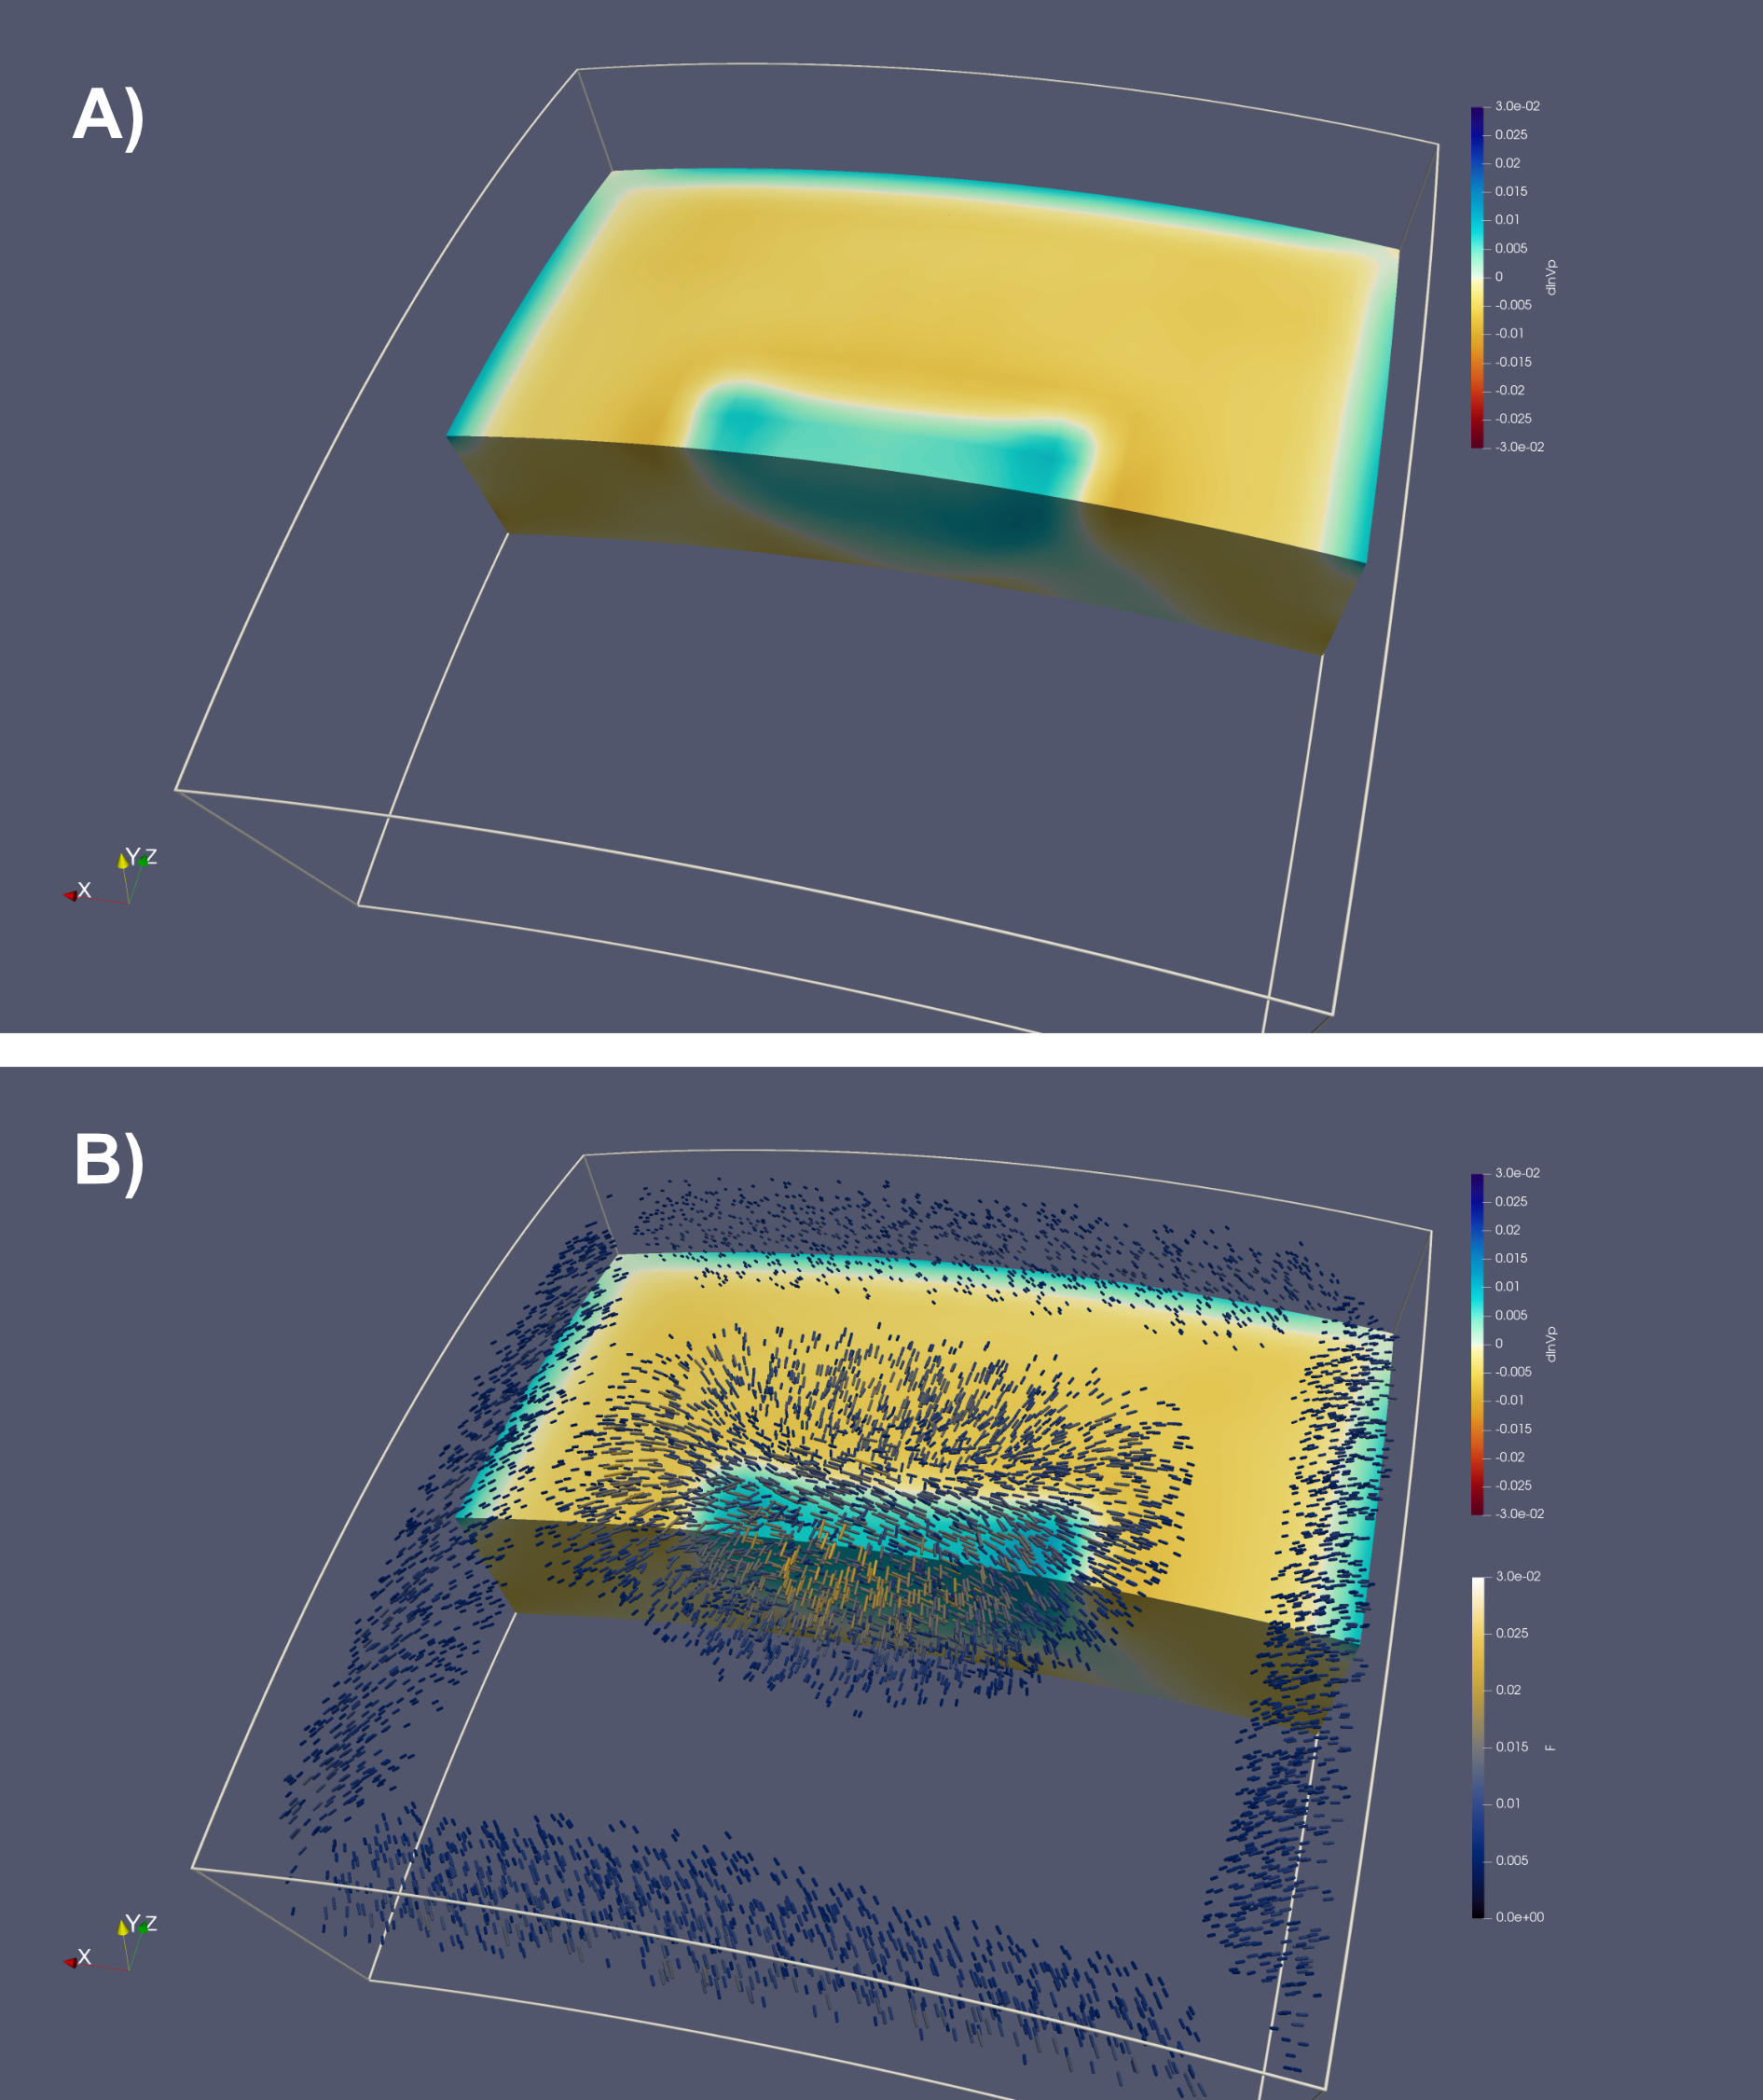
\includegraphics{PSI_D/PSI_D_Results.png}
    \caption{Sinking Slab tomography example. A) Isotropic inversion of P-wave travel-times. B) Anisotropic inversion of P and S travel-times and S splitting intensity. In both panels, the recovered isotropic P-wave anomaly is contoured and the model is sliced through the center of the sinking slab at 300 km depth and in the east-west direction; full extent of the model is outlined. In B), a random distribution of recovered hexagonal symmetry axes (i.e. fast axes) are plotted and colored by the anisotropic strength. Symmetry axes are shown only where the anisotropic strength is >0.5\%.\\
    }
    \label{fig:psi_d_results}
\end{figure}

\subsection{Subducting Plate}
In addition to the Sinking Slab example, we also include the files required to reproduce the anisotropic tomography results for the subducting plate shown in Figure \ref{fig:radial+sks} (or Figure 9 of the \textbf{ECOMAN} publication) and reproduced below in Fig. \ref{fig:psi_d_subduction}. The inputs required to run the inversion are located in \path{examples/SubductingPlate}. The reference \viztomotitle{} model file is not included due to its large size. To run the inversion, do \texttt{julia jl-files/run\_inversion.jl}. The results will be stored in \path{psi_output/ANI_TTP_TTS}. This inversion should finish in approx. 15 minutes. Once finished, load the state-file \path{visualization/render_model.pvsm} in \textbf{Paraview} (be sure to update the path to the appropriate output directory when prompted by the \textbf{Paraview} dialog box) and the tomographic results should appear as show in Fig. \ref{fig:psi_d_subduction}.

\begin{figure}[ht]
    \centering
    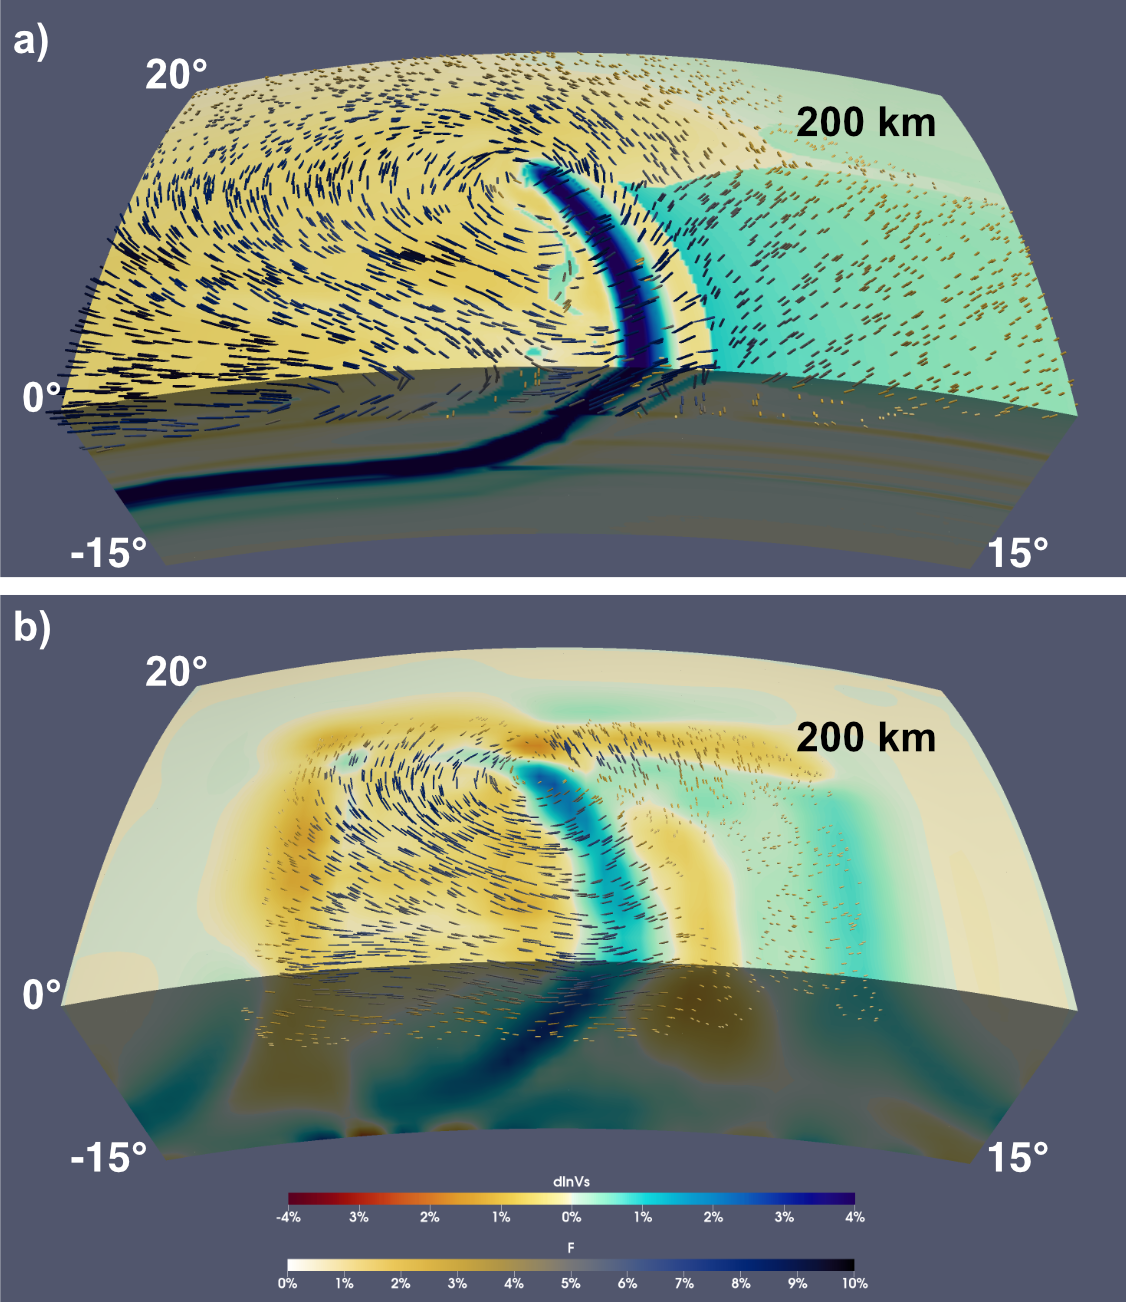
\includegraphics{PSI_D/PSI_D_Subduction.png}
    \caption{Synthetic subducting plate example. (a) Target anisotropic model generated from VIZTOMO. (b) Recovered anisotropic model obtained by inverting synthetic teleseismic P and S (relative) travel times computed from the model in (a). In both panels, the isotropic S-wave velocity perturbations are computed with respect to the far-field 1D velocity profile. Quivers parallel the hexagonal symmetry axis and are scaled and coloured by the anisotropic strength. The top surface shown is located at 200 km depth while the full model extends from 0-1000 km along the radial direction, 85°-115° along longitude, and 0-20° along latitude.\\
    }
    \label{fig:psi_d_subduction}
\end{figure}


% REFERENCES
% Aki, K., Christoffersson, A., \& Husebye, E. S. (1977). Determination of the three‐dimensional seismic structure of the lithosphere. Journal of Geophysical Research, 82(2), 277-296.

% Bezada, M. J., Faccenda, M., \& Toomey, D. R. (2016). Representing anisotropic subduction zones with isotropic velocity models: A characterization of the problem and some steps on a possible path forward. Geochemistry, Geophysics, Geosystems, 17(8), 3164-3189.

% Bodmer et al. (2020)

% Lévêque, J. J., \& Masson, F. (1999). From ACH tomographic models to absolute velocity models. Geophysical Journal International, 137(3), 621-629.

% Masson, Y., \& Romanowicz, B. (2017). Box tomography: localized imaging of remote targets buried in an unknown medium, a step forward for understanding key structures in the deep Earth. Geophysical Journal International, 211(1), 141-163.

% Munzarová, H., Plomerová, J., \& Kissling, E. (2018a). Novel anisotropic teleseismic body-wave tomography code AniTomo to illuminate heterogeneous anisotropic upper mantle: Part I—Theory and inversion tuning with realistic synthetic data. Geophysical Journal International, 215(1), 524-545.

% Paige, C. C., \& Saunders, M. A. (1982). LSQR: An algorithm for sparse linear equations and sparse least squares. ACM Transactions on Mathematical Software (TOMS), 8(1), 43-71.

% Schmandt, B., \& Humphreys, E. (2010). Seismic heterogeneity and small‐scale convection in the southern California upper mantle. Geochemistry, Geophysics, Geosystems, 11(5).

% Toomey, D. R., \& Foulger, G. R. (1989). Tomographic inversion of local earthquake data from the Hengill‐Grensdalur central volcano complex, Iceland. Journal of Geophysical Research: Solid Earth, 94(B12), 17497-17510.

% Toomey, D. R., Solomon, S. C., \& Purdy, G. M. (1994). Tomographic imaging of the shallow crustal structure of the East Pacific Rise at 9$^{\circ}$30′ N. Journal of Geophysical Research: Solid Earth, 99(B12), 24135-24157.

% VanderBeek \& Faccenda (in review)